\documentclass{article}

\usepackage{amsthm}
\usepackage{amsmath}
\usepackage{cite}
\usepackage{listings}
\usepackage{multicol}
\usepackage{url}
\usepackage{graphicx}
\graphicspath{ {./imgs/} }

\setlength{\parindent}{4em}
\setlength{\parskip}{1em}


\begin{document}

\pagenumbering{gobble}

\begin{center}
  \textbf{Project Progress Report}

  \textit{Derick Anderson and Harshitha Bhaskar, Blackboard: AndersonBhaskar}
\end{center}

\section*{Idea}

The core idea of the project is to develop a journaling tool for managing your
reading. Functionality will include, for example, the ability to track your
progress through books from want-to-read to finished, write reviews of books,
and organize books by author and series. To support said functionality will
require a data model for books, authors, reading lists, etc.

We love to read, but lose track of all the information to do with our
reading. It is great to be able to look forward to the things you want to read,
look back on the things you’ve read, and organize your thoughts about your
reading.

\section*{Response to Feedback/Questions}

We have decided to use MySQL instead of SQLite.

Derick has extensive experience with Python,
but no experience with MySQL
except that gained through this class.

Harshitha has extensive experience with MySQL, gained from and outside this class, 
but, has only just learnt Python and does not have much experience with it.

A small set of data will be manually curated to demonstrate the functionality of
the system.

\section*{UML and EER Diagrams}

\begin{figure}[h]
  \centering
  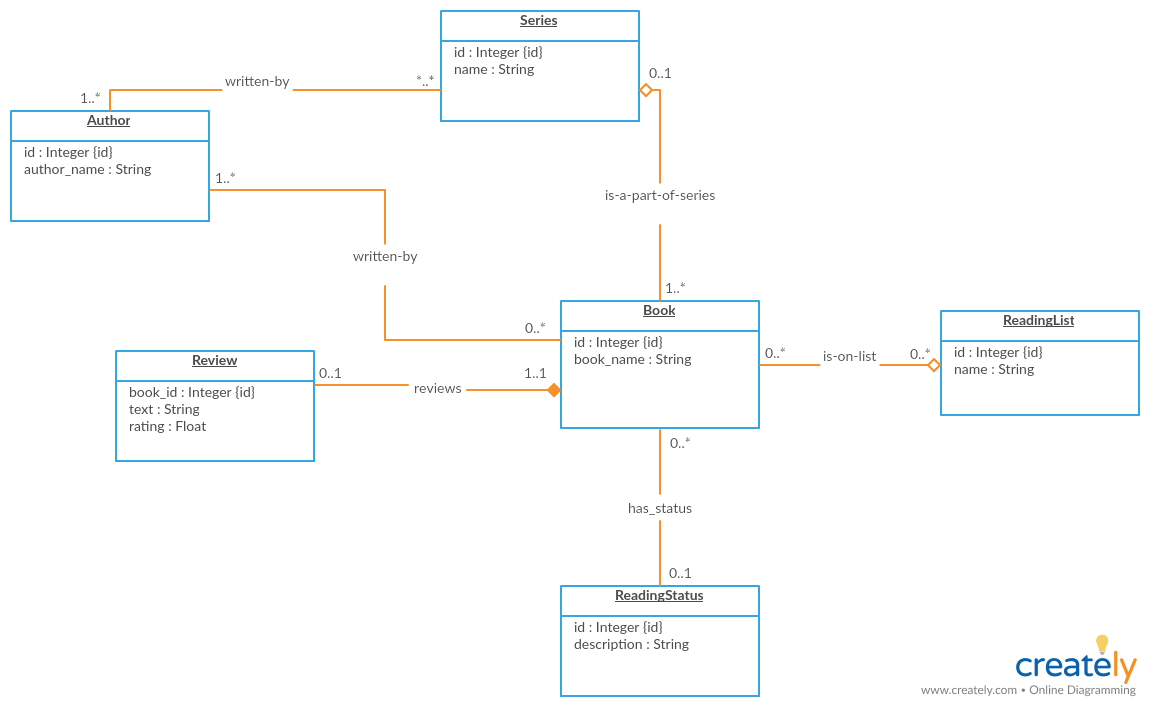
\includegraphics[width=\textwidth]{uml}
  \caption{UML Diagram}
\end{figure}

\begin{figure}[h]
  \centering
  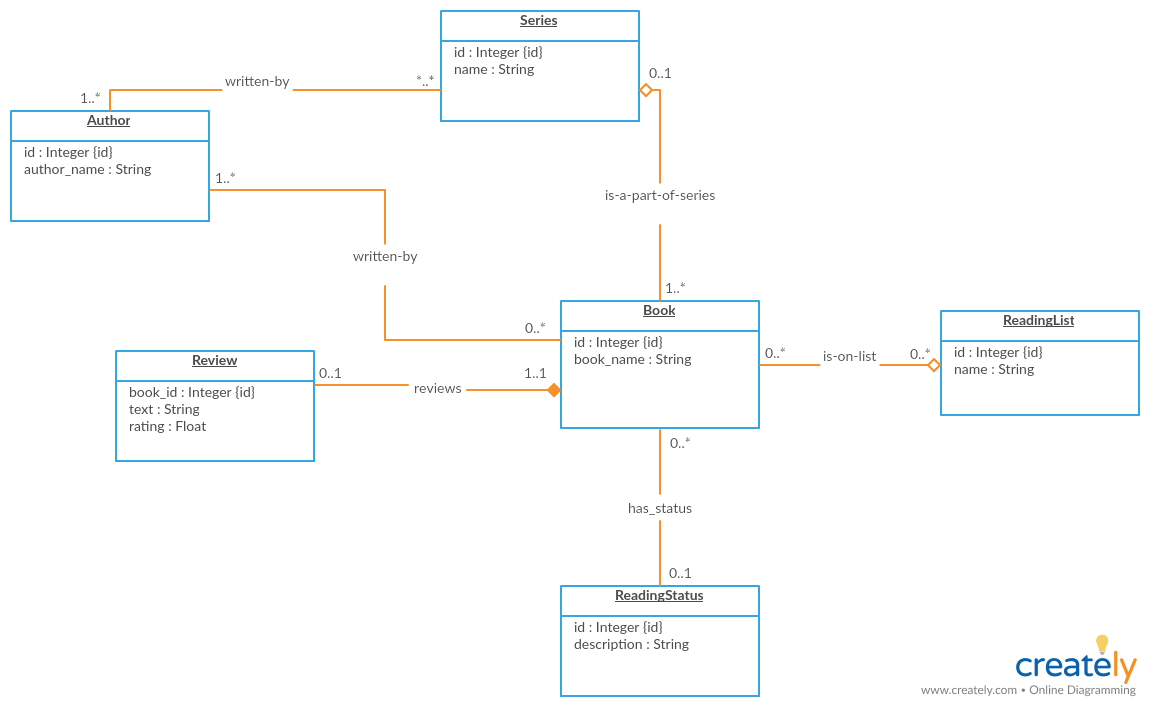
\includegraphics[width=\textwidth]{uml}
  \caption{EER Diagram}
\end{figure}

\section*{Sample User Interaction}

When the user launches the app, the UI will contain 4 buttons at the header which 
represent how you wish to sort your reading list by series("Sort by Series"), just 
view your entire reading list in chronological order ("Sort by Reading List") or 
to view reading list based on ratings of books ("Sort by Ratings"). The user can 
click on either of these. If neither is clicked, the default view is chronological. 
Along with this re-grouping functionality, user also has access to 2 more buttons 
that returns your reading list as just book names ("Books") and books along with 
reviews ("Reviews").

The reading list is displayed as a list with columns "Book Name", "Date Started", 
"Date Ended", "Rating", "Review".

To add a book to the reading list, the only required data is the name of the book 
and start date. 
An "Add Book" button will be available towards the top right corner of the page. 
Clicking this triggers a pop-up box to enter book name, date started, date ended, 
rating and review. As stated before. only book name and date started are required 
to be entered. Once submit is clicked, the book is added chronologically to the 
list of books.

\section*{Technical Specifications}



\end{document}
%%% Local Variables:
%%% mode: latex
%%% TeX-master: t
%%% End:
